\documentclass[a4paper,10pt]{article}
\usepackage[utf8x]{inputenc}
\usepackage{array}
\usepackage{graphicx}
\usepackage{float}

%opening
\title{Generalized Top Down Parsing In Cubic Time}
\author{Arnold Lankamp}

\begin{document}

\maketitle

\begin{abstract}

In this article we will describe a generalized top down parsing algorithm. Since it's top down it will be easier for a human to understand. Additionally we will also demonstrate that, in terms of efficiency, our implementation performes excellent.

\end{abstract}

\section{Introduction}

If the abstract didn't catch your attention yet, here are some highlights:
\begin{itemize}
 \setlength{\itemsep}{0pt}
 \setlength{\parskip}{0pt}
 \setlength{\parsep}{0pt}

 \item Worst case cubic space and time bounds with respect to the length of the input.
 \item Worst case linear scaling relative to the size of the grammar.
 \item Linear performance on LL(k) and LR(k) grammars.
 \item No performance hit for rules that are not left factored.
 \item Generating or hand crafting the parser code is trivial.
 \item Parse traces are easy to follow; using a debugger to step through the parse process can actually be informative.
 \item Low constant overhead.
\end{itemize}
We call our parser, the Scannerless Binary Forest Generalized Top Down Parser or SBFGTD (BF also means Bloody Fast, in case your wondering why it was put in the abbreviation).

\section{Recognizer}

TODO: Write chapter introduction.

\subsection{GSS}

As is common in generalized parsing, we use a kind of Graph Structured Stack (GSS). In our case we generate a stack node with a unique identifier for every symbol in the grammar. So for for example; if we would have the following grammar: $S\,::=\,AB\,|\,BA,\,A\,::=\,a,\,B\,::=\,b$, we would assign identifiers as follows: $S$(-1), $A$(0), $B$(1), $B$(2), $A$(3), $a$(4) and $b$(5). Every terminal and non-terminal on the right hand side of a production gets a unique identifier, regardless whether or not a comparable right hand side occurs again in another position in the grammar. These identifiers are needed to handle sharing in the GSS correctly. Each stack node consists of this identifier, edges back to their 'parents' and information about it's 'right neighbour' in the production, so we know where to go next.

Since the GSS only contains nodes that we expect to 'encounter', there are at most $O(N)$ of them; one of every type per location in the input string. Since a node only has one edge to each of it's possible parents per level and there are $O(N)$ levels, there are at most $O(N)$ edges per node. This means that the total algorithm becomes $O(N^3)$. In the worst case there are $N$ times $O(N)$ nodes that match a substring that ends in the current level; when moving to the 'next' node in the production all edges of these nodes need to be carried over, this time this operation needs to complete is equal to the number of levels before the current position (so $N$ at most), hense $O(N)\,*\,N\,*\,N\,=\,O(N^3)$.

\subsection{Basic algorithm}

\begin{enumerate}
 \setlength{\itemsep}{0pt}
 \setlength{\parskip}{0pt}
 \setlength{\parsep}{0pt}

 \item Expand the left most node of every production that did not match anything yet on all stacks, until no stacks can be expanded anymore (i.e. they all have a terminal at the bottom).
 \item Match all nodes on the bottom of the stacks to the input. Reduce the ones that match, remove the ones that don't.
 \item Reduce the nodes on all stacks that matched something and have them queue the 'next' node in the production they are part of where applicable, until no reductions are possible anymore.
 \item goto 1.
\end{enumerate}

\subsection{Pseudocode}

{\small
\begin{verbatim}
parse(){
  toExpandSet.push('startNode');
  expand();
  
  do{
    reduce();
    expand();
  }while(toReduceSet.notEmpty());
  
  if(notAtEOI()) parse error;
}

expand(){
  while(toExpandSet.notEmpty()){
    node = toExpandSet.pop();
    
    Node[] children = getChildrenFor(node);
    for(childNode <- children){
      if(reducedStore.contains(childNode)){ // Child already has results
         if(notAddedEarlierInThisLoop){ // Sharing
           toReduceSet.add(node);
         }
      }else{
        if(expandedStore.contains(childNode)){ // Sharing
          expandedStore.get(childNode).addEdge(node);
        }else{
          expandedStore.add(childNode);
          
          if(childNode.isTerminal()){
            toReduceSet.push(childNode);
          }else{
            toExpandSet.push(childNode);
          }
        }
      }
    }
  }
}

reduce(){
  while(toReduceSet.notEmpty()){
    node = toReduceSet.pop();
    reducedStore.add(node);
    
    if(node.hasEdges()){
      for(parent <- node.edges){
        if(toReduceSet.notContains(parent) &&
            reducedStore.notContains(parent)){ // Sharing (is reduced)
          toReduceSet.push(parent);
        }
      }
    }else if(node.hasNext()){
      next = node.next;
      if(toExpand.contains(next)){ // Sharing
        next = toExpandSet.get(next);
      }else if(expandedStore.notContains(next)){ // Sharing
        toExpandSet.push(next);
      }
      next.addEdges(node.edges);
    }
  }
}
\end{verbatim}
}

\subsection{From grammar to code}

Writing or generating the recognizer / parser code is relatively strait forward. All that it needs is a direct translation from the grammar rules to either functions or some kind of table like data structure. Basically it just needs to know what alternatives are associated with a each non-terminal. In case we are generating code, this would mean that one function per non-terminal is needed, which contains logic that informs the recognizer / parser about what alternatives should be expected.

Since the mapping between the original grammar and the code or table is one-on-one, it is even possible to implement or edit it by hand without much effort. Another advantage is that, in combination with the top-down-ness of our algorithm, it makes tracing errors in a grammar easier; if you'd want to know why something doesn't match at a certain position, you can just go through it with a debugger to see what happens. Your degree of success naturally depends on the amount of stacks that are alive at the moment you're trying to observe, but at least the possibility to do so exists.

\subsection{Example traces}

To illustrate how the recognizer works, here are some example traces.

\subsubsection{Strait forward}
$S\,::=\,AB$\\
$A\,::=\,a$\\
$B\,::=\,b$\\
input = $ab$

\begin{enumerate}
 \setlength{\itemsep}{0pt}
 \setlength{\parskip}{0pt}
 \setlength{\parsep}{0pt}
 
 \item expand S
 \item expect AB
 \item expand A
 \item expect a
 \item reduce a and follow edge to A
 \item move from A to B
 \item expand B
 \item expect b
 \item reduce b follow edge to B
 \item reduce AB and follow edge to S
 \item reduce S
 \item done.
\end{enumerate}

\subsubsection{Left recursive}
$S\,::=\,A$\\
$A\,::=\,Aa\,|\,a$\\
input = $aaa$

\begin{enumerate}
 \setlength{\itemsep}{0pt}
 \setlength{\parskip}{0pt}
 \setlength{\parsep}{0pt}
 
 \item expand S
 \item expect A
 \item expand A
 \item expect Aa $|$ a
 \item expand A $\Rightarrow$ A shared
 \item reduce a and follow edge to A
 \item move from A to a
 \item reduce Aa and follow edges to S and A
 \item parse for S is incomplete and is discarded
 \item move from A to a
 \item reduce Aa and follow edges to S and A
 \item parse for S is complete.
 \item move from A to a
 \item reduce Aa failed, since EOI has already been reached.
 \item done.
\end{enumerate}

TODO: Maybe convert to illustrations?

\section{Parser}

\subsection{Parse forest}

To represent the parse forest we use a format that was especially designed for this parser, to ensure worst-case behaviour remains within cubic time and space bounds. We call it 'deflattenized', for lack of a better description; it's intent is similar to binarization, but it's implementation is somewhat different.

The parse forest consists of nodes. Every node in the forest contains a 'result', which represents a substring for a certain terminal or non-terminal. In case of non-terminals, these 'results' contain one or more references to alternative representations of the substring it denotes. Each node also contains a set of prefixes. A prefix only consists of a reference to a node. If you trace all possible paths through the prefixes of a node to the start, you'll get all alternatives for a certain production at a certain location.

Every node in the tree is identified by the substring it represents and it's prefixes; all the prefixes of a certain node denote the same substring, which end were the 'result' contained in the node starts. All prefix sets are shared regardless of the node's end position that they are matched to, so there are at most $O(N)$ of them. Every prefix set can contain up to $N$ different prefixes. Since there can be only one 'result' per substring, this means there are at most $O(N^{2})$ 'results'. Overall this makes the parse forest $O(N^{3})$ worst-case, since the number of unique nodes is limited to $O(N^{3})$. We'll look into this with more detail further on in this chapter.

Additionally it is possible to output a flattened version of the parse forest at the user's request. Naturally this parse forest will be unbound polynomial in size in the worst-case. Pratically this unlikely to happen; moreso since filtering can be done during parsing and flattening, making it improbable that many ambiguities remain in the final tree. We'll discuss filtering later on in this document.

\subsubsection{Example}

Parse tree example:
Grammar:
$S\,::=\,AAAA\,|\,AAA\,|\,AA$\\
$A\,::=\,a\,|\,aa$\\
input = $aaaa$

\begin{figure}[H]
\centering
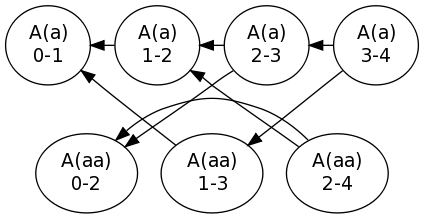
\includegraphics[width=0.5\textwidth]{a_aa-forest.png}
\caption{A partial visual representation of the parse forest, showing all alternatives for '$S0$-$4$'. The numbers indicate start and end position of the matched substring.}
\end{figure}

\begin{table}[H]
\centering
\begin{tabular}{ p{15em} p{15em} }
Derivation & Forest path\\
\hline
S(A(a),A(a),A(a),A(a)) & $A0$-$1$ $\leftarrow$ $A1$-$2$ $\leftarrow$ $A2$-$3$ $\leftarrow$ $A3$-$4$\\
S(A(a),A(aa),A(a)) & $A0$-$1$ $\leftarrow$ $A1$-$3$ $\leftarrow$ $A3$-$4$\\
S(A(aa),A(a),A(a)) & $A0$-$2$ $\leftarrow$ $A2$-$3$ $\leftarrow$ $A3$-$4$\\
S(A(a),A(a),A(aa)) & $A0$-$1$ $\leftarrow$ $A1$-$2$ $\leftarrow$ $A2$-$4$\\
S(A(aa),A(aa)) & $A0$-$2$ $\leftarrow$ $A2$-$4$
\end{tabular}
\caption{'Flattened' version of the parse forest}
\end{table}

\subsubsection{Worst case example}

Worst-case parse tree example:

Grammar:\\
$S\,::=\,SSS\,|\,SS\,|\,a\,|\,\epsilon$\\
input = $a\,*\,1\,-\,a\,*\,10$

\begin{table}[H]
\centering
\begin{tabular}{ | p{6em} | p{4em} | p{4em} | p{4em} | p{3em} | p{5em} | }
  \hline
  Input length & Results & Nodes & Pointers & Total & Total / $N^{3}$ \\
  \hline
  0 & 2 & 2 & 3 & 7 & - \\
  1 & 5 & 6 & 9 & 20 & 20 \\
  2 & 8 & 13 & 15 & 36 & 4.5 \\
  3 & 11 & 24 & 21 & 56 & 2.074 \\
  4 & 14 & 40 & 27 & 81 & 1.265 \\
  5 & 17 & 62 & 33 & 112 & 0.896 \\
  6 & 20 & 91 & 39 & 150 & 0.694 \\
  7 & 23 & 128 & 45 & 196 & 0.571 \\
  8 & 26 & 174 & 51 & 251 & 0.490 \\
  9 & 29 & 230 & 57 & 316 & 0.433 \\
  10 & 32 & 297 & 63 & 392 & 0.392 \\
  \hline
\end{tabular}
\caption{Worst-case parse tree data}
\end{table}

\subsection{Psuedocode}

Augmenting our regonizer with parse tree construction code it trivial. Only a few minor adjustments are needed.

{\small
\begin{verbatim}

Parser psuedocode:
parse(){
  toExpandSet.push('startNode');
  expand();
  
  do{
    reduce();
    expand();
  }while(toReduceSet.notEmpty());
  
  if(notAtEOI()) parse error;
  
  return findResultStore('startNode');
}

expand(){
  while(toExpandSet.notEmpty()){
    node = toExpandSet.pop();
    
    Node[] children = getChildrenFor(node);
    for(childNode <- children){
      if(reducedStore.contains(childNode)){
        findResultStore(node).
            addAlternative(childNode.prefixes, childNode.results);
        if(notAddedEarlierInThisLoop){ // Sharing
          toReduceSet.add(node);
        }
      }else{
        if(expandedStore.contains(childNode)){ // Sharing
          expandedStore.get(childNode).addEdge(node);
        }else{
          expandedStore.add(childNode);
          
          if(childNode.isTerminal()){
            toReduceSet.push(childNode);
          }else{
            toExpandSet.push(childNode);
          }
        }
      }
    }
  }
}

reduce(){
  while(toReduceSet.notEmpty()){
    node = toReduceSet.pop();
    reducedStore.add(node);
    
    if(node.hasEdges()){
      for(parent <- node.edges){
        findResultStore(parent).
            addAlternative(node.prefixes, node.results);
        if(toReduceSet.notContains(parent) &&
            reducedStore.notContains(parent)){ // Sharing (is reduced)
          toReduceSet.push(parent);
        }
      }
    }else if(node.hasNext()){
      next = node.next;
      if(toExpandSet.contains(next)){ // Sharing
        next = toExpandSet.get(next);
      }else if(expandedStore.notContains(next)){ // Sharing
        toExpandSet.push(next);
      }
      next.addEdges(node.edges);
      next.updatePrefixes(node.prefixes, node.results);
    }
  }
}

findResultStore(node){
  return resultStores.
    findOrCreate(node.startLocation, node.endLocation, node.name);
}

\end{verbatim}
}

NOTE: algorithm / psuedocode was reverse engineered from the actual implementation and has been made more generic. (I'm currently unsure whether or not I accidentially ommitted any special cases in the conversion).

\section{Optimizations}

The basic algorithm is fairly strait forward and relatively simple to implement. The naïve implementation will respect worst-case cubic time and space bounds, however adaptations can be made to improve its overall efficiency.

\subsection{General}

Making the implementation breath first / level synchronized generally reduces resource usage. This is because it enables us to determine when certain data is no longer necessary and can be discarded. Additionally, since much information is stored on a per-level basis we can exploit the assumption that we are level synchronized to our advantage. For example, the memory used for stacks that died off can be reclaimed and reused and sharing and such can be handled slightly more efficiently.

Another minor performance improvement can be made by matching on entire literals at once, instead of on characters. This decreases the amount of necessary GSS nodes and thus reduces stack activity.

A more obivious optimization is adding support for look-ahead filtering. Simply by adding simple checks to the parser code, we can prevent unnecessary work; if a certain alternative will never match, we don't need to expect it. The number of characters we look ahead is not limited, by theoretical of practical constraints.

\subsection{Edge related}

Generally parsers store results on edges in the GSS; likely for convenience reasons. If we would refrain from doing this and store parse results elsewhere (in a table with constant look-up time), edges could remain pointers. At first sight this may not be an advantage, however we would be able to share edges among GSS nodes and it opens up numereous other interesting opportunities for optimization.

First of all, by caching 'expected children' for every type of node per level a substantial performance increase can be achieved. Namely, this will ensure linear scaling for non-left-factored grammars. The reason for this is the following; for example, if we take the grammar rule: $E\,::=\,E\,+\,E\,|\,E\,-\,E$. The expansion at the first level would look like this:
\begin{enumerate}
 \setlength{\itemsep}{0pt}
 \setlength{\parskip}{0pt}
 \setlength{\parsep}{0pt}
 
 \item $E$(0) $\rightarrow$ $E$(1) $+$ $E$(2)
 \item $E$(1) edges = {$E$(0)}
 \item $E$(0) $\rightarrow$ $E$(3) $-$ $E$(4)
 \item $E$(3) edges = {$E$(0)}
 \item $E$(1) $\rightarrow$ $E$(1) $+$ $E$(2)
 \item $E$(1) edges = {$E$(0), $E$(1)}
 \item $E$(1) $\rightarrow$ $E$(3) $-$ $E$(4)
 \item $E$(3) edges = {$E$(0), $E$(1)}
 \item $E$(3) $\rightarrow$ $E$(1) $+$ $E$(2)
 \item $E$(1) edges = {$E$(0), $E$(1), $E$(3)}
 \item $E$(3) $\rightarrow$ $E$(3) $-$ $E$(4)
 \item $E$(3) edges = {$E$(0), $E$(1), $E$(3)}
\end{enumerate}
Clearly demonstrating quardratic behaviour. If we would remember what the edges set of one $E$, we can reuse it for any other $E$ in the same level and update it with additional edges by reference; this is possible since nodes are guaranteed to have the same edges if they are 'expected' by the same 'parent(s)'. This will make the expansion look like this:
\begin{enumerate}
 \setlength{\itemsep}{0pt}
 \setlength{\parskip}{0pt}
 \setlength{\parsep}{0pt}
 
 \item $E$(0) $\rightarrow$ $E$(1) $+$ $E$(2)
 \item $E$(0) $\rightarrow$ $E$(3) $-$ $E$(4)
 \item $E$ edges = {$E$(0)}
 \item $E$(1) $\Rightarrow$ $E$ edges += $E$(1)
 \item $E$(3) $\Rightarrow$ $E$ edges += $E$(3)
\end{enumerate}
Now expanding clearly completes in linear time. An additional benefit is that all the edge sets are shared between the children of the different $E$'s, saving memory. It will reduce the worst-case number of edges to $N\,*\,\mathit{numberOfLHS's}$. Originally this would have been $N\,*\,\mathit{numberOfProductions}^{2}$, so this is a massive improvement. One additional benefit is, that this optimization lessens the need for left-factoring of grammars. In absence of look-ahead filtering performance should be on par with the non-factored equivalent of the grammar; in cases where look-ahead information is used, it may be close enough to remove it's necessity.

Finally, we can also gain something at the other end. The 'is reduced' check on nodes can be eliminated. Since every GSS node of the same 'sort' always has exactly the same children if they are in the same level, it is sufficient to initially just follow the first edge in an edge set. In case the node this edge points to has already been reduced in this level, nothing needs to be done (except record the alternative, in case we're parsing and not just recognizing); otherwise all other edges need to be followed as normally would have been the case. Since this guarantees a node can never be queued for reduction more then once, we can remove the check. This improves performance by a factor between one and the number of non-terminals in the grammar.

\subsection{GSS}

In many grammars productions exist that start with the same symbols. There is no reason to do duplicate work for these symbols. For example, if we take the grammar rule: $S\,::=\,E\,+\,E\,|\,E\,-\,E$. Both $E$'s at the start of these productions will always be derived exactly the same way for the same substring(s) and thus they are equal. Because of this, the prefixes of these two productions may as well be merged; i.e. by converting the rule into $S\,::=\,E\,(+\,E\,|\,-\,E)$. It is trivial to modify our algorithm to support this. Simply by allowing every node in the GSS to have more then one 'next' node and assigning the same id to both $E$'s (to indicate they must be shared), the desired result can be achieved. Naturally the shared prefixes of grammar rules can be arbitrarily long and are not restricted to just two partially equal rules; as long as a rule's prefix overlaps with another rule it can be shared, regardless whether or not it already has been shared with another rule. This optimization ensures we can recognize and parse LR(k) grammars using just one stack, thus in linear time without any overhead.

\section{Filtering}

TODO: Write chapter introduction.

\subsection{Follow restrictions}

Follow restrictions are trivial to implement. They work as a kind of look-ahead after the production; if the production we are trying to reduce matches the specified character(s) after the current location in the input, the reduce fails.

\subsection{Rejects}

Any alternative can be marked as reject. It this reject alternative matches, all other alternatives this reject belongs to are discarded. Rejected nodes are partially removed from the GSS at parse time and partially during post-parse filtering / flattening. Removing rejected stacks while parsing prevents unnecessary work from being performed; however it can be expensive to do in case the node at the end of the rejected alternative's edge is already reduced. This is the reason why it's not completely at parse time.

Reject alternatives may be nested, however they are not allowed to be cyclic, since this may lead to incorrect behaviour. Consider the following grammar: $S\,::=\,A\,|\,B,\,A\,::=\,B(r)\,|\,a,\,B\,::=\,A(r)\,|\,a$. The reject edges are marked with $(r)$. The order in which reductions are done will determine the final parse result. For example, we could follow the edge from $A$ to $B$ first and reject $B$; since $B$ is rejected it won't be reduced, so $A$ won't be rejected as we don't follow the edge from $B$ to $A$ and we end up with $S(A(a))$. On the other hand the opposite may happen and we'd end up with $S(B(a))$. So in practice it may, or may not do what you intended.

TODO: Check, consider, rewrite and such; there may be something wrong with rejects in certain cases in the current implementation (i.e. nested rejects that contains subtrees that have an alternative path to an ambiguous reject higher up in the tree may show unwanted behaviour).

\subsection{Priorities and associativity}

Priorities and associativity restrictions are implemented as 'don't nest' relation. For example, if we take the grammar rule $E\,::=\,E\,*\,E\,>\,E\,+\,E$, this means that the production $E\,+\,E$ can't be a child of the production $E\,*\,E$ on either side of the production. Similarly $E\,::=\,E\,+\,E\,\{left\}$ means that the production $E\,+\,E$ can't be a child of itself on the left side of the production; similarly for $\{right\}$, but the other way around. If declared as $\{nonassoc\}$ it can't be nested on either side of itself.

The current implementation handles priority and associativity filtering completely at parse time. While reducing it checks whether or not the reduction is allowed for the edge we want to follow; in case it is, it's stored in a result node that is identified by the sort name of the node the edge points to and the key that indicates which other non-terminals with the same sort name have the same set of 'don't nest' relations. This is done to preserve sharing in the resulting tree. For example consider the following grammar rule: $E\,::=\,E(1)\,*\,E(2)\,\{left\}\,>\,(E(3)\,+\,E(4)\,|\,E(5)\,-\,E(6))\{left\}$. Here $E(3)$ and $E(5)$ would share the same result nodes while parsing, just as $E(4)$ and $E(6)$, since their 'don't nest' relations are identical.

\subsection{Actions}

Each grammar rule can have a number of actions associated with it. These actions can be used to disambiguate non-context-free ambiguities or filter alternatives that can't be disambiguated using priorities. I won't go into detail about this feature, since it's not an integral part of the parser, but more of a post-parse filter.

\section{Benchmarks}

In this chapter we will have a look at the performance of you current implementation of the algorithm.

Benchmarks were executed on a machine with the following specifications:
\begin{table}[H]
\centering
\begin{tabular}{ | p{6em} | p{9em} | }
 \hline
 CPU & Q6600 \\
 Memory & 8 GB DDR-800 \\
 OS & Fedora Core 12 \\
 JRE & Sun 1.6.0\_13 (32-bit) \\
 JRE options & -Xmx1g \\
 \hline
\end{tabular}
\end{table}

Measurements are listed in terms of CPU-time (system + user time) and are gathered using Java's build in management tool. Before performing the benchmarks, the recognizer / parser code was ran a number of times, so the JIT compiler had the opportunity to optimize.

\subsection{Worst case}

The obvious candidate for a benchmark is the following worst-case grammar:
$S\,::=\,SSS\,|\,SS\,|\,a$\\
input = $a\,*\,50\,-\,a\,*\,500$

\begin{table}[H]
\centering
\begin{tabular}{ | p{5em} | p{7em} | p{6em} | }
  \hline
  Input chars & Recognize Time & Parse Time \\
  \hline
  50 & 4 & 6 \\
  100 & 18 & 36 \\
  150 & 60 & 130 \\
  200 & 154 & 332 \\
  250 & 322 & 672 \\
  300 & 596 & 1206 \\
  350 & 996 & 2018 \\
  400 & 1534 & 3184 \\
  450 & 2228 & 4776 \\
  500 & 3090 & 6880 \\
  \hline
\end{tabular}
\caption{Worst-case performance scaling; times are in milliseconds.}
\end{table}

\begin{figure}[H]
\centering
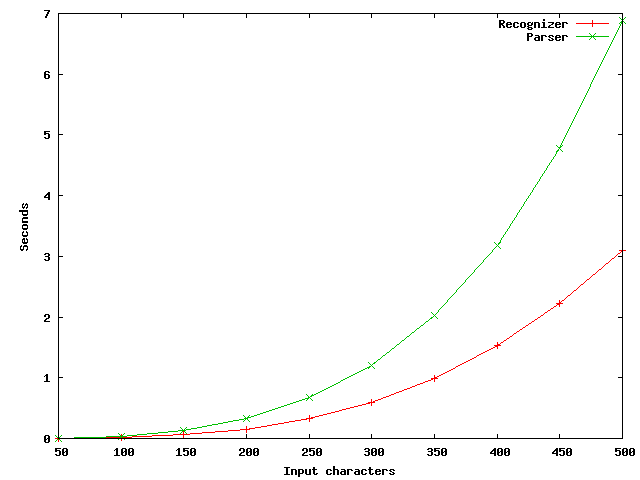
\includegraphics[scale=0.5]{worst-case.png}
\caption{Worst-case recognizer and parser performance scaling.}
\end{figure}

Note however that the recognizer is optimized for speed and the parser for a balance between memory usage and speed (meaning a faster implementation is possible). Regardless of this, it clearly demonstates (close to) cubic worst-case behaviour, as expected. Looking at the times, our implementation seems very efficient in worst-case scenarios.

\subsection{Grammar factoring}

Apart from worst-case behaviour in terms of the number of ambiguous parse results, it is also interesting too look at how well we perform on worst-case grammars without ambiguous input. Here we will compare the performance of our parser between different version of a grammar; a non-factored version, a left-factored version and a prefix-shared version. The original grammar is the following:\\
$S\,::=\,A+$\\
$A\,::=\,a\,|\,E$\\
$E\,::=\,1\,|\,E\,+\,E\,|\,E\,-\,E\,|\,E\,*\,E\,|\,E\,/\,E\,|\,E\,>\,E\,|\,...$ 25 more like it ...\\
input = $a\,*\,50000\,|\,a\,*\,100000\,|\,a\,*\,150000\,|\,a\,*\,200000$

It contains lots of left-recursion and one non-ambiguous path. So one would expect non-linear performance in this case. However, as can be seen in the graph below this is not the case. Performance seems to scale perfectly linear regardless of how the grammar is factored.

TODO: Change grammar and text. Bottom up (GLR) parsers are likely also linear on this one.
TODO: Highlight differences between different kinds of factoring.

\begin{figure}[H]
\centering
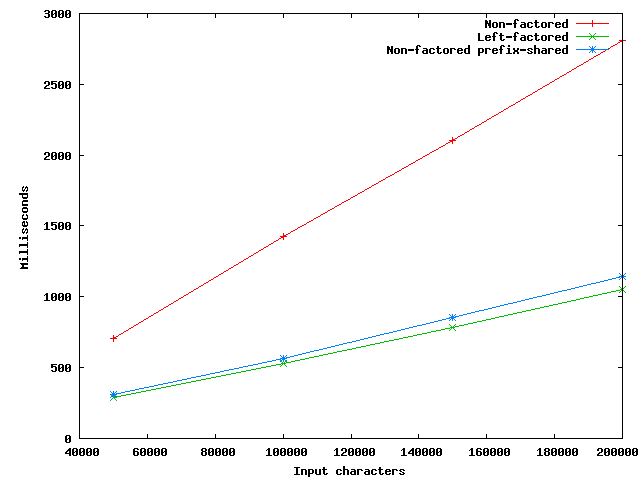
\includegraphics[scale=0.5]{grammar-factoring.png}
\caption{Grammar factoring related parse time scaling; without look-ahead.}
\end{figure}

\end{document}
